\documentclass[12pt]{article}


\usepackage[numbers]{natbib}
\usepackage{graphicx} 
\usepackage{amssymb, amsmath, amsthm} 
\usepackage{fontenc} 
\usepackage{amscd,latexsym,amsfonts,amstext,amsbsy}
\usepackage{euscript} 
\usepackage{enumerate} 
\usepackage{color}  
\usepackage{physics}
\usepackage[latin1]{inputenc}
\usepackage{tikz}
\usepackage{mathrsfs}
\usetikzlibrary{shapes,arrows}
\usepackage{multicol}
\usepackage{comment}
\usepackage{color,soul}
\usepackage{combelow}
\usepackage{tabu}
\usepackage{caption}
\bibliographystyle{apa}
\definecolor{applegreen}{rgb}{0.55, 0.71, 0.0}




\textwidth = 16 cm
\textheight = 24 cm
\oddsidemargin = 0.0 cm
\evensidemargin = 0.0 cm
\topmargin = -2 cm
\parskip = 0.2in
\parindent = 0.0in


\newtheorem{theorem}{Theorem}
\newtheorem{problem}[theorem]{Problem}
\newtheorem{exercise}[theorem]{Exercise}
\newtheorem{corollary}[theorem]{Corollary}
\newtheorem{lemma}[theorem]{Lemma}
\newtheorem{proposition}[theorem]{Proposition}
\newtheorem{proporties}[theorem]{Proporties}
\newtheorem{definition}[theorem]{Definition}
\newtheorem{definitions}[theorem]{Definitions}
\newtheorem{example}[theorem]{Example}
\newtheorem{remark}[theorem]{Remark}

 


\begin{document}
\textbf{\large{Modeling the Heroin Epidemic}} \\
Suzanne Lenhart, Tricia Phillips, Christopher Strickland \\
\today \\

\textcolor{blue}{Blue font: contains questions I have, things to discuss.} \\
\textcolor{red}{Red font: things I am working on/need to do.} \\ 
\textcolor{red}{Reminder for me: use present tense, use powerful/direct language.} \\
\textbf{Abstract} \\ \\
\textcolor{red}{Fill in after write paper.} \\ \\
\textbf{Introduction} \\ \\
\textcolor{red}{Want to ``funnel in": start with general epidemic information and then narrow in on the drugs involved.}\\ \\
\textcolor{green}{General opioid epidemic} \\
\textcolor{red}{Re-order to better fit funnel with ``all" stats first, then prescription opioids, then heroin, then fentanyl (follows flow of people better, too)} \\
\textcolor{red}{Fill in stats from various sources in below paragraphs.} \\
\textcolor{red}{Find motor vehicle vs. drug overdose stats} \\


\textcolor{red}{Start of stats about opioid epidemic at large to begin paragraph:} The misuse of opioids, including prescription pain relievers, synthetic opioids, and the illegal drug heroin, is rampant in today's society \cite{NIH2}. The opioid crisis was declared a public health emergency in October 2017 by the United States Department of Health and Human Sciences \cite{HHS1}. It was estimated that the total economic cost of prescription opioid dependence, abuse and overdoses in 2013 alone was \$78.5 billion \cite{Florence}. \textcolor{red}{Put in idea about how fentanyl has become leading cause of overdoses, etc.} Due to the health risks of the addicted individuals, public health concerns, the number of overdose deaths and the economic burden, this is an issue worth paying attention to.

\textcolor{blue}{Statistics regarding heroin and why we should care:} \\
A national survey estimated that out of the United States national population of individuals of 12 years of ago or older, 948,000 were heroin users in 2016, although this number may include under-reporting \cite{CDC2}. There were an estimated 13,219 heroin deaths in 2016, a more than six-fold increase from the year 2002, despite there being roughly half as many heroin users in 2002 \cite{NSDUH1}. This, in part, is due to the recent trend of lacing heroin with fentanyl \textcolor{red}{(put in background on fentanyl)}, a surgical-grade opioid that is up to fifty times more potent than heroin alone, and therefore, users are unaware of the purity of the heroin they obtain \cite{CDC1, NIH2, Volkow2}. \textcolor{red}{Find source regarding purity of heroin trends/graphs for past few decades.} The effects of heroin, however, extend further than just the specific individual using the drug. Due to the sharing of needles and other equipment involved in the injection of heroin, the human immunodeficiency virus (HIV) and the hepatitis C virus (HCV) are more easily contracted as transmittance occurs through bodily fluids. In addition, risky sexual behavior is heightened under the influence, so addicts have an increased risk of transmitting and contracting these viruses. Women who use heroin during pregnancy put their babies at risk for neonatal abstinence syndrome in which the drug is passed along to the baby, resulting in dependency and thus, withdrawal symptoms upon birth \cite{NIDA2}. 

\textcolor{green}{Prescription opioid information} \\
\textcolor{blue}{About prescription opioids and why we should care:} \\
Another large portion of opioids consist of prescription pain relievers which are either natural (morphine and codeine), semi-synthetic (oxycodone, hydrocodone, oxymorphone), or synthetic, (fentanyl, tramadol) \cite{CDC3, TNMentalHealth2}. From 1991 to 2011, there was a near tripling of prescriptions that pharmacies distributed \cite{NIDA1}. This was in part due to a number of new opioids that were approved by the FDA for use, such as OxyContin, Actiq, Fentora, and Onsolis (fentanyl), in addition to other unapproved opioid products for pain management \cite{FDA1}. Moreover, in the early 2000s, drug manufacturers funded publications and physicians to support opioid use for pain control \cite{Mandell}. A national survey estimated there were 11.5 million individuals of 12 years of age or older in the United States that experienced pain reliever misuse in the past year, referring to the year 2016 \cite{CDC2}. In this survey, misuse was defined as taking the prescription at a higher dose, more frequently or longer than prescribed, taking someone else's medication, or any other way not directed by a doctor \cite{SAMSHA3}. Misuse of prescription pain relievers occurs for a variety of reasons and the same survey asked individuals who reported prescription pain reliever misuse to give the reason and the source for their most recent misuse. The most prominent responses for reasons of misuse were to relieve physical pain, to feel good or get high, and to relax or relieve tension. The largest source was from friends/relatives or from a healthcare provider, followed by given a prescription or stolen from a health care provider \cite{CDC2}. Options for treatment of opioid addiction involve medications such as buprenorphine, methadone, and naltrexone, in combination with counseling and behavioral therapies \cite{SAMSHA1}. In addition, pregnant women who take prescription opioids also put their babies at risk of neonatal abstinence syndrome, similar to heroin \cite{CDC5}. 


\textcolor{green}{Connection between opioid and heroin abuse} \\ \\
\textcolor{blue}{Transitioning from prescription opioids to heroin:} \\
The misuse of prescription pain relievers leads some individuals to start heroin. According to the National Survey of Drug Use and Health (NSDUH) survey information from 2002-2011, nearly 80\% of heroin users reported non-medical prescription pain reliever use prior to their heroin use. Here, non-medical prescription use is defined as taking prescriptions that were not prescribed to the user directly or used only for the feelings it causes. In fact, those who had prior non-medical prescription pain reliever use were 19 times more likely to initiate heroin use than those without prior use \cite{Muhuri}. This could in part be due to the higher availability of heroin in recent years at a lower cost than alternative opioids \cite{NIDA1}. Moreover, approximately 3.6 percent of non-medical prescription pain reliever users began using heroin within 5 years of their first opioid; although a small percentage, this is a significant number of individuals given the magnitude of opioid addiction \cite{Muhuri}. In 2010, an abuse-deterrent formulation of the commonly abused prescription opioid OxyContin was released that made abuse through injection and inhalation more challenging. Although done with the intent of reducing opioid abuse, studies showed that many individuals switched to heroin use instead \cite{Cicero2, Cicero3}. One study of young adults ages 18-25 concluded that among many factors including race, education status, martial status, other drug use, as well as many others, the use of non-prescribed opioid pain relievers in the past year was the biggest indicator of an individual using heroin in the past month, past year or in their lifetime \cite{Ihongbe}. Comparing NSDUH data from 2002-2004 and 2008-2010, the average yearly rates of past year heroin use increased among non-medical opioid users, but heroin use stayed static for those who reported no non-medical use of opioids; the highest rate of heroin use was among individuals with past year non-medical use of opioids ranging between 100 and 365 days of use \cite{Jones}. In the 1960's, heroin users were composed mainly of younger, nonwhite men in urban areas with their initial opioid being heroin, but in recent decades, this trend has shifted to older, white, rural and suburban men and women with their initial opioid being a prescription \cite{Cicero}. Opioids are of no shortage in society today and since opioid addiction is driven largely by legal prescription medication availability, this has made a significant proportion of society susceptible to misuse and addiction to opioids, including heroin. 

\textcolor{green}{Heroin information} \\ \\
\textcolor{blue}{About the drug} \\
Heroin is an illicit drug classified as an opioid and comes in the form of a white or brown powder or as a black substance resembling roofing tar. The drug is injected, sniffed, snorted or smoked and quickly enters the brain to bind to opioid receptors. It provides the user with feelings of euphoria, in addition to physical effects such as heavy feelings in the arms and legs, dry mouth, and sometimes nausea and vomiting \cite{NIH1, NIDA2}. There are short and long term negative effects on the body for using the drug, and consequently, it is currently considered a schedule I drug, meaning that there is no approved medical use of heroin and there is a high likelihood for abuse. \cite{DEA1, NIH1}. Addicted individuals have withdrawal symptoms such as restlessness, diarrhea, vomiting, and cold flashes, along with cravings for the drug which makes stopping use of the drug very difficult \cite{NIH1}. Treatment options for heroin use are the same as for prescription opioids \cite{SAMSHA1, NIH1}. Heroin users build up a tolerance to the drug with repeated use and can overdose on the drug, in which their heart rate and breathing is slowed to a dangerous level without medical assistance \cite{NIDA2, NIH1}. Due to built-up tolerance, the risk of overdose is high when individuals stop their use of the drug for a period of time (i.e. while in recovery or hospitalized) and return to use. This is because they may return to the previous amount they were taking before, without knowing what their body can currently tolerate \cite{NIH2}.  


\textcolor{green}{Other models} \\ \\
\textcolor{blue}{Previous models involving heroin} \\
\textcolor{red}{``Group" other models after 4 sentences of White and Comiskey (for paper). Say ``other models include..." or ``Approaches also include...agent-based modeling, etc." Or ``of interest is..." to cut down on length significantly (cut out all details for paper, keep for dissertation)} \\
\textcolor{red}{Look for fentanyl use/addiction models, if any} \\
There have been several models formulated focusing on heroin addiction. Most of them were motivated by and extensions of the White and Comiskey ordinary differential equation model with three compartments each representing a different stage as a drug-user: the susceptible class including individuals aged 15-64, the drug user class composed of individuals not in treatment, and finally, the drug users in treatment. In this model, individuals in treatment for drug use were only able to die, relapse to drug use, or complete treatment and be immune to drug use for the remainder of the modeling time period. The basic reproduction number, $\mathscr{R}_0$, was calculated and deemed most sensitive to the rate of individuals in the susceptible class becoming drug users; therefore, prevention is more important than treatment for reducing drug use \cite{White}. Wang, Yang and Li did analysis of this model, changing the assumption that the population was not constant \cite{Wang}. 

%\textcolor{blue}{Question: How can the model assume the three compartments make up the entire population, but then have the option for immunity to drug addiction for the remainder of the modeling period? Answer: NOT necessarily the same people; just equal number of people (i.e. someone is born susceptible to replace someone who became immune, maybe)  

The White and Comiskey model was modified later on by Liu and Zhang in order to incorporate a relapse distribution in which there was a non-constant time to relapse. They formulated a delay-differential equation, and also took away the assumption that the population was constant. Their conclusions about the sensitivity of $\mathscr{R}_0$ to certain parameters were in line with those from White and Comiskey \cite{Liu}. Using the same three compartments, another model was formulated with the idea of the relapse rate relying on the length of time the individual has been undergoing treatment. This coupled ODE-PDE model assumed that susceptibles could only become addicted via interaction with heroin users not undergoing treatment. Prevention was deemed more important than treatment, yet again \cite{Fang1}. Fang, Li, Martcheva and Caialso (2015) also modeled the heroin epidemic allowing susceptibility of becoming a drug user to depend on age, again resulting in a coupled ODE-PDE model \cite{Fang2}. A non-autonomous version of the White and Comiskey model included a distributed time delay for becoming a drug user along with both the parameters and the total high-risk population size being time-dependent \cite{Samanta}. From this, an autonomous model was developed incorporating the distributed time delay, which was converted into a discrete model with the time step-size being one \cite{Abdurahman}. Finally, a three compartment model consisting of susceptibles, users not in treatment, and those in treatment, assumed that those not in treatment could not recover and return to being susceptible, and that it took two contacts with a drug user to become addicted, resulting in a nonlinear incidence rate; results showed that perhaps the heroin prevalence undergoes periodic changes depending on conditions \cite{Ma}. 
%\textcolor{blue}{Question: Should I go through each paper specifically, like I have above, or moreso "group them" by stating some ways that the White and Comiskey model was modified and then reference them all together?} Answer: do them individually, that's better 

A deviation from the three compartmental model was done that included a fourth compartment which consisted of individuals who successfully recovered from their heroin use, whether through deciding to stop use by themselves or via treatment measures \cite{Wangari}. The treatment of heroin users is limited by the availability of treatment facilities and resources and therefore, a saturated treatment function is incorporated; the saturation parameter was concluded as having the most vital role in the persistence of the epidemic. This implies that intervention is important early on before heroin addicts accumulate in the community and thus, prompt treatment is necessary. 
 %http://journals.plos.org/plosone/article/file?id=10.1371/journal.pone.0102263&type=printable) 
Another model consisting of 84 ODE's captured the dynamics between prescription opioid users with acute pain, those with chronic pain, illicit opioid users, heroin users and those who overdose. Results showed that increasing addiction treatment and reducing prescriptions for individuals with chronic pain seemed to have a greater impact on reducing both heroin overdose deaths and the number of opioid abusers compared to reducing prescriptions for acute pain without treatment increases \cite{Benneyan}. \textcolor{red}{This was from a conference preceding...in future, look for published model from Benneyan.} 

%\textcolor{blue}{Question: Should only include population level models, correct...not something like a heroin market model (agent-based) with drug users, sellers, homeless \& police?} Will put in that model, and can do anything related because if those authors are editors, they will not like if they don't see their own work referenced. 

Others have taken a completely different approach, specifically using agent-based modeling. In addition to their ODE model, Benneyan, Garrahan, Ilie\cb{s}, and Duan (2017) formulated two agent-based models: the first being a cellular automata model consisting of a grid with neighboring cells updated depending on state variables adjacent to the cells; the second being a network model with nodes that represent individuals/subpopulations and weighted pathways dependent on relational strength and nearness. \textcolor{red}{Not all variables are defined, such as P(x,y), so look for full model from Benneyan when published.} The former was to better understand regional spread and the latter to investigate spread among individuals; their results suggested that with various regulation practices for opioids, heroin death rates would decrease, but the authors recognize the reality of unintended consequences of these legislations \cite{Benneyan}. Agar (2001) created an agent-based model, consisting of a world with 2,500 patches and 100 agents each assigned an experimentation value which defines how likely that individual is to experiment with heroin, depending on their interest in trying something new, their attitude toward illicit drug use, and their desire to follow societal rules. The model was able to track the number of heroin experimenting individuals over time with the agent moving randomly, one patch selected at random to contain heroin in the beginning, and the ability for individuals to obtain heroin from their original patch, from others who have experimented, or from another patch where the transferring of heroin between agents occurred \cite{Agar}. \textcolor{red}{Put in brief explanation of ``Reducing the complexity of an agent-based local heroin market model" paper by Heard. \\ } \\

\textcolor{blue}{Summary of Christopher's opioid paper and why formulating another model:} \\
\textcolor{red}{Need to update with new revisions/any new results from final version that's published!} The motivation for our heroin model comes from a previous model focusing on opioid addicts through prescriptions and via the black market \cite{Battista}. In order for the model to have an addiction-free equilibrium, both addictions that come from prescriptions and addictions from accessibility to excess prescription drugs must be eliminated, which equates to the need for close administration and monitoring of those prescribed. Furthermore, near the addiction-free state, the prevention of prescription opioid users becoming addicted is more important for staying near the addiction-free equilibrium than reducing the number of prescriptions getting into the hands of non-prescribed users. \textcolor{red}{Fix wording:} However, away from the addiction-free state, a realistic situation, the most important factors in reducing the number of addicted individuals include increasing the prescription completion rate, increasing entry into treatment (even among low success rates), and decreasing the prescription rate. The purpose of formulating a separate model from this prescription opioid model is to be able to understand the more complicated dynamics that arise among opioid addiction with the addition of heroin/fentanyl use. \textcolor{red}{Make the case for the new model clearer: want to emphasize how we need new model because of fentanyl being the biggest killer now and with putting in a heroin/fentanyl class, this could lead to different management strategies.} As exemplified previously, heroin and fentanyl play a significant role in the process of opioid addiction and recovery and so it's inclusion provides a more accurate overall picture of the epidemic. \textcolor{red}{Read clarifying definitions again:} From 2000-2015, there were fewer heroin overdoses compared to prescription opioid overdoses but around 2010, a sharp increase of heroin overdoses occurred primarily due to the involvement of fentanyl. Therefore, it is crucial to take a more detailed look at this increasing problem \cite{CDC4}. \textcolor{red}{Regarding overdoses: study directly.} Moreover, we alter how the recovery process is viewed, by thinking about those in recovery still as addicts, and not having the ability to become a susceptible individual again. 


\textcolor{blue}{How our model is different than previous models:} \\
\textcolor{red}{Include details on how my model different than previous ones.} \\
 \textcolor{red}{Took out ``heroin history," so need to incorporate argument regarding why we constructed a data-driven model versus a theoretical model as done in the past (i.e. use recent data changes as an argument, especially with increase in fentanyl}. Previous models have not incorporated the connection between prescription opioid misuse and heroin or fentanyl use at all, instead focusing solely on heroin addiction and recovery. Although there are many factors that play a role in population size, susceptibility to drug use, relapse time and other parts of the drug-using process, we consider individuals in each of the classes to be homogeneous, for simplicity of a starting model. \textcolor{red}{discussion of how our model differs from the prescription opioid model: best to differentiate throughout the paper} \\
 \textcolor{red}{Provide argument/connect to info before for why the problem is so large now that we need data-driven models compared to just a theoretical heroin addiction model as done for decades.}


\textcolor{green}{Goal paragraph} \\ \\
\textcolor{blue}{Goals for our model/questions trying to answer:} \\
To address this apparent problem in today's society, we model the prescription opioid/heroin/fentanyl epidemic in order to understand the dynamics behind the epidemic and predict the trajectory of the epidemic. We identify important conditions relating to the reduction of opioid/heroin/fentanyl addiction. To do that, we have formulated a population level system of ordinary differential equations model consisting of classes of individuals taking prescription opioids, addicted to opioids, using heroin or fentanyl, and successfully recovered from addiction to opioids, heroin and/or fentanyl, and analyzed it. Our overall goal is to explore how different management strategies may alter the epidemic trajectory; specifically, we would like to investigate management strategies for optimally treating pain with prescriptions while reducing opioid, heroin, and fentanyl addiction.


\textbf{Model Formulation} \\ \\
To the extent of our knowledge, there have been no mathematical models incorporating both prescription opioid addiction and heroin/fentanyl addiction. Although terminology is not always clearly defined in the literature, such as opioid misuse, abuse, dependency, addiction and use disorder, we aim to focus on addiction only, where addiction to opioids is defined as having a pattern of continued non-medical use that is already, or could be, harmful \cite{Vowles}. We take opioid use disorder to fall in this categorization of addiction, due to the definition presented in \cite{SAMSHA2} which includes sustained use regardless of interference with life obligations. Our model consists of five subgroups of a population, in which they are all proportions of the entire population: 

1. Susceptibles $S$: This portion of the population consists of individuals who are not taking prescription opioids of any kind, nor using heroin or fentanyl. \\ \\
2. Prescription opioid users $P$: This class of individuals consists of individuals who are prescribed opioids by a health care provider and take the opioids at a level that is not considered addicted. We note that individuals in this class could be misusing prescription opioids, but not at the level of addiction.  \\ \\ %"Misuse" in data: questions may ask about misuse in the past 12 months, and so even 1 time of misuse would count 
3. Opioid addicts $A$: This group of individuals are addicted to opioids, but not using heroin or fentanyl, or are actively in treatment for opioid addiction. For individuals who go to treatment for opioid addiction, they remain in this class for at least 4 weeks \textit{after} being discharged from treatment; if they relapse within 4 weeks after treatment, they are again considered addicted and can remain in this class for longer. (Although the opioid class of drug includes heroin and fentanyl, here we take opioids to mean non-heroin and non-fentanyl.) \\ \\
4. Heroin/fentanyl users $H$: This class is composed of individuals who are addicted to heroin or fentanyl, or are actively in treatment for heroin/fentanyl addiction. For individuals who go to treatment for heroin/fentanyl addiction, they remain in this class for at least 4 weeks \textit{after} being discharged from treatment; if they relapse within 4 weeks after treatment, they are again considered addicted and can remain in this class for longer. (We note that individuals in this class could be using other drugs or are addicted to opioids in addition to heroin or fentanyl, but they are at least addicted to one of these drugs). \\ \\
5. Recovered individuals $R$: This class consists of individuals who completed treatment for opioid or heroin/fentanyl addiction and did not relapse within 4 weeks after treatment, and therefore are considered in a ``stable" recovery state.  

\textcolor{blue}{Clarifications on definitions:}
We include illicit fentanyl users in the class of heroin users, because of the potency of the drug, which is what those addicted to prescription opioids seek--lower cost and a better high. In addition, a portion of those who overdose from the very powerful drug fentanyl are individuals who are using heroin that is laced with it; therefore, the use of fentanyl is oftentimes intertwined with the use of heroin. There is much variability in the purity of heroin due to the lacing of the drug with fentanyl, and 1 in 5 overdose deaths have multiple drugs present so it is difficult to know the actual cause of death \cite{CDC4}. We believe it is difficult to separate the use of heroin and fentanyl, so putting them in the same class is the most natural choice. Finally, we remark that use of heroin is implicitly understood to be addictive due to the highly addictive nature of the drug, and we assume no casual use of the drug \cite{NIH1}. If an individual uses heroin at a level that it would be easy to stop using, they are better classified as a susceptible individual rather than a heroin addict, based on the definition of addiction we are using. Similarly, individuals who use fentanyl outside of short-term, carefully monitored settings with a health provider is assumed to be addicted. \textcolor{red}{Source for fentanyl addictive nature, length of time of prescription short?} We try to take into account these complexities as best as possible with the information in literature.

We denote the initial conditions as
$S(0)=S_{0}$, $P(0)=P_{0}$, $A(0)=A_{0}$, $H(0)=H_{0}$, and $R(0)=R_{0}$, and we assume all of these values are positive. The initial values for each of the classes are proportions of the entire population \textcolor{red}{and therefore are dimension-less...add this to parameter/unit table in appendix.}

 
Here, we present our ordinary differential equation model:
\[\dv{S}{t} = -\alpha S - \beta_{A} SA  -\beta_{P} SP- \theta_{1} SH +\epsilon P +\mu (S+P+R+A+H) + \mu_{A}A + \mu_{H} H -\mu S \quad (1)\] 
\[\dv{P}{t} = \alpha S - \epsilon P  - \gamma P - \theta_{2}PH- \mu P    \quad(2)\]
\[\dv{A}{t} = \gamma P + \sigma R \frac{A}{A+H+\omega} +\beta_{A} SA  +\beta_{P} SP -\zeta A - \theta_{3}AH-(\mu + \mu_{A})A   \quad (3)\]
\[\dv{H}{t} = \theta_{1}SH+\theta_{2}PH+\theta_{3}AH + \sigma R \frac{H}{A+H+\omega}-\nu H-(\mu+\mu_{H})H  \quad (4)\]
\[\dv{R}{t} = \zeta A +\nu H -\sigma R \frac{A}{A+H+\omega}-\sigma R \frac{H}{A+H+\omega} -\mu R\quad(5)\]
\vspace{.05cm}
\[S+P+A+H+R=1 \quad(6).\]
\textcolor{red}{See if best way to write this last equation?}

\textcolor{red}{Why can we assume this sum is 1?...short time frame, population constant; we are imposing because population not changing so much (i.e. we made the model to be this way/work out this way mathematically)} We assume that these five compartments sum to one, so that the population is of constant size, i.e. the total death rate is equal to the incoming rate for the susceptible class.  Since these rates are the same, $\mu S$, equation (1) simplifies to: 

\[\dv{S}{t} = -\alpha S - \beta_{A} SA  -\beta_{P} SP- \theta_{1} SH +\epsilon P +\mu (P+R)+ (\mu + \mu_{A})A + (\mu+\mu_{H}) H \quad (1)\] 


The parameters involved in this model represent transition rates from one class to another and are per capita yearly rates:
\begin{itemize}
\item $\alpha S$: rate at which susceptible individuals are prescribed opioids (1/year) \textcolor{red}{May change to be clearer in each of these parameters about the units (i.e. per prescription user year or whatever it is) or may just leave that for the parameter table where units are listed}
\item $\beta_{A} SA$: rate at which susceptible individuals become addicted to opioids by black market drugs or interaction with other addicts (1/year)
\item $\beta_{P} SP$ : rate at which susceptible population obtains extra prescription opioids and becomes addicted  per year
\item $\theta_1 SH$: rate at which susceptible population becomes addicted to heroin or fentanyl by black market availability or interaction with other heroin or fentanyl users  (1/year)
\item $\epsilon P$: rate at which individuals return to the susceptible class after being prescribed opioids and did not develop an addiction (1/year) 
\item $\mu S, \mu P, \mu A, \mu H, \mu R$: natural death rates (1/year)
\item $\mu_A A$: enhanced death rate for opioid addicts; overdose rate which results in death (1/year)
\item $\mu_H H$: enhanced death rate for heroin or fentanyl addicts; overdose rate which results in death (1/year)
\item $\gamma P$: rate at which prescribed opioid users become addicted to opioids (1/year)
\item $\theta_2 PH$: rate at which prescribed opioid users become addicted to heroin or fentanyl (1/year)
\item $\sigma R \frac{A}{A+H+\omega}$: rate at which individuals transition from the recovered class into the opioid addicted class which is proportional to the approximate proportion of individuals in the recovered class that came from A that are relapsing back to that class. We include a perturbation term $\omega$ here in the case that $A$ and $H$ are both 0, such as in the addiction-free case. (note: even though we do not know where individuals came from originally, we make the assumption that individuals go back to their primary drug of choice/the reason they entered treatment, so relapse back approximately proportional to where they came from \textcolor{red}{Source/explanation below..also, fix wording when take care of this depending on what we go with. Also mention that this is an approximation because it's based on the ``current time" class proportions (not the time step when they went to R). We are doing this because the percentages/stats we are using are ``relapse rates" so that means individuals are going back where they started.}) (1/year)
\item $\zeta A$: rate at which addicted opioid users enter treatment/rehabilitation (1/year)
\item $\theta_3 AH$: rate at which the opioid addicted population becomes addicted to heroin or fentanyl  (1/year)
\item $\sigma R \frac{H}{A+H+\omega}$: rate at which individuals transition from the recovered class into the heroin/fentanyl addicted class which is proportional to the approximate proportion of individuals in the recovered class that came from A that are relapsing back to that class. We include a perturbation term $\omega$ here in the case that $A$ and $H$ are both 0, such as in the addiction-free case. (note: even though we do not know where individuals came from originally, we make the assumption that individuals go back to their primary drug of choice/the reason they entered treatment, so relapse back approximately proportional to where they came from \textcolor{red}{Source below..also, fix wording when take care of this.}) (1/year)
\item $\nu H$: rate at which heroin or fentanyl users enter treatment/rehabilitation 
\end{itemize} 
%Recovery--1 month: those in treatment experience acute withdrawal, after 1 month: post-acute (emotional freight train) 
%potentially make theta1=theta2 to reduce the number of parameters
%Look at pain management articles and why people relapse. 
%Get intuition about potential arrows from papers. 

\textcolor{blue}{Clarification of some aspects of the model:} \\
We note that although sellers are not directly involved in the model nor have to be addicts themselves, addicted individuals act as a proxy for sellers of the drug and general availability of the drug, whether it is opioids or heroin. This is because the higher number of addicted individuals there are, the more sellers there needs to be which results in an increased exposure to the drug and therefore, increased chance of addiction. Although treatments for addictions are an enormous problem in and of themselves since there is limited success as shown by the parameter values for the recovery rates, we are acknowledging treatments as a part of recovery in our model, but do not go into specifics for this first model. We are classifying overdoses to mean opioid overdose-related deaths (i.e. not from secondary factors or long term effects). Although overdose death data includes both accidental and non-accidental deaths (i.e. suicide, assault), we assume here that if an individual died from an overdose-related death, they were addicted \textcolor{red}{see calculation in appendix; I don't think we assume this anymore from \cite{Gwira} information} (i.e. the number of intentional deaths is negligible). \textcolor{red}{This is CDC definition (from data packet) is for prescription opioids and fentanyl; see if also same for heroin.}
%https://pep-c.rti.org/HERO/KB/Documents/CDCs\%20Opioid\%20Overdose\%20Indicator\%20Support\%20Toolkit.pdf%
We also note the fact that Naloxone, an overdose-reversing medication, has saved individuals from overdoses, but \cite{NIDA2} \textcolor{red}{make some argument that the number saved is negligible compared to the number of overdoses, so we assume results in death most of the time.}\\ 

\textcolor{blue}{Explanation of different R class, how different from Christopher's opioid paper:} \\
\textcolor{red}{Fix: don't want to use ``negative" language such as ``we did something to \textit{avoid} someting else," etc. Reword so saying something like ``Other choices for dealing with recovery include..., two recovery classes, etc...} \\
We note that the terms $\sigma R \frac{A}{A+H+\omega}$ and $\sigma R \frac{H}{A+H+\omega}$ were included in order to avoid having two recovered classes, which would prevent the transition of individuals who recovered from one drug to initiate use of the other (or if we included those pathways, would become too complicated for a first model). One study suggested that 10\% of the prescription opioid addicts they followed up with post-treatment had used heroin at least five times in the previous year, which demonstrates the importance of keeping these transitions as possibilities \cite{Weiss}. We decided to define a recovered class instead of a recovery class as the model presented in \cite{Battista} did, because the recovery class would have consisted of two very different groups of individuals: those with a high chance of relapse (e.g. recently finished treatment) and those with a much lower chance of relapse (e.g. successfully finished treatment in the past and has remained free of addiction for a significant amount of time). This definition of the recovered class creates a compartment to place individuals who have been addicted in the past and have finished treatment but are not considered actively addicted anymore and should be dealt with differently than susceptible individuals, those in treatment, and those recently out of treatment. %This definition of a recovered class is also beneficial when it comes to the data; data for the number of addicted individuals would include those in recovery, so our class avoids having to parse out how many are in recovery versus not in recovery.  \\ 

\textcolor{blue}{Support/data/arguments for why choosing 4 weeks/acute withdrawal period} \\
\textcolor{blue}{Summarize these multiple supporting sources into a few sentences and only go into this much detail in disseration?}
We choose to use 4 weeks after treatment with no relapse as the mark of when people are ``successfully recovered" and can move to R. We chose this time frame due to several studies exhibiting a high level of relapse within weeks of discharge from treatment, which suggests individuals are not stably recovered. One study following up with opiate dependent individuals (of which 88\% of the study population were heroin users) showed that 59\% of the individuals discharged from treatment relapsed within 1 week and 71\% within 4 weeks \cite{Smyth}. Moreover, 80\% of individuals who relapsed after treatment did so within 4 weeks and that 92\% of individuals who relapsed after discharge had gone back to treatment prior to their follow-up interview (which was between 18-42 months). These statistics convey the unstable nature of an addicts' recovery, particularly within a few weeks of post-treatment (since that's when a majority of them relapsed). In another opiate dependent group study evaluating their relapse risk, 27\% had relapsed on the discharge day of their most recent treatment program, 41\% had relapsed within 1 week and 65\% within 4 weeks \cite{Bailey}. The only study found specifically for prescription opioid addicts suggested that 91\% of them who completed a two-phase treatment program relapsed back into addiction within 8 weeks post-treatment \cite{Weiss}. On the lower side, in another study an estimated 32\% of the 68 opiate addicts interviewed returned to addiction within 4 weeks and 65\% lapsed, which we note has potential to lead to dependence in time; at the 6 month follow-up, 50\% of the 60 individuals interviewed were dependent \cite{Broers}. Another study following up with opiate users post-treatment for 6 months showed that 32\% had lapsed within 1 week post-discharge when interviewed; 71\% had lapsed by the 6th week; and 44\% had returned to the daily use of opiates (considered addicted) at the 2 month mark. Furthermore, the study stated that several individuals who completed the withdrawal portion of the program lapsed while in the second, in-patient part of treatment (although not necessarily equating to a full relapse back into addiction) which supports our claim that those who entered treatment addicted should be still be considered addicted while in treatment \cite{Gossop1}. Later analysis of this study regarding relapse factors stated that 25\% of those who lapsed mentioned withdrawal symptoms as playing a role in their lapses \cite{Gossop2}. These statistics suggest that opiate-abstinence can be difficult to achieve in this initial time period post-treatment: ``...the period immediately after leaving a residential treatment is of massively high risk: the great majority of lapses occurred with the first few weeks after discharge...after the first four weeks, there were few additional lapses...first few weeks after discharge as a \textit{critical period} in the process of recovery" \cite{Gossop1}. This suggests four weeks can be viewed as an important marker in recovery, and that individuals who bounce back to addiction/frequently relapse in this time frame should simply remain in their respective addicted classes. Other studies suggest significant lapse and relapse rates within weeks and months for heroin addicts and opiate addicts, as well \cite{Hunt, Gossop3}. \\
Therefore, since 71\% of heroin addicts relapse within 4 weeks post-treatment and an estimated 91\% of prescription opioid addicts in recovery relapse back to addiction within 8 weeks post-treatment (the majority most likely within four weeks based on these other studies), we keep these individuals in the addiction class since they have not fully ``recovered," i.e. at a point where they are less likely to fall back into addiction \cite{Weiss, Smyth}.

\textcolor{blue}{Information on relapse coming from primary drug and not source-driven, argument for form of our transition terms being proportional to number in each addicted class} \\
In one study, 63\% of initial lapses occurred around other opioid users, 48\% in another addicts' home, and 31\% in ones own home \cite{Gossop1}. This may lead one to believe that interactions with other addicts would play a large role with an initial lapse/relapse; however, following this study, the authors explored the circumstances that led to the lapses of these study subjects and results proved differently. The top factors that led to these initial lapses were cognitive factors (planned to use), mood states (angry, sad, lonely, etc.), and external influences (situations unrelated to drug use that led to use). This was taking into consideration the number of people who mentioned the factors, the total number of times the factors were mentioned, the number of individuals who deemed the factor most important, and finally, the number of individuals that indicated the factor was the initiator of a sequence of other factors, as lapse often is a result of multiple factors occurring simultaneously. These were also the factors that were primarily contributed to the continued use of opiates. It seems clear that source-driven factors, specifically social pressure (offered drugs), drug availability (in another users' home or in the area), drug-related clues (objects used for drug-taking/observing others under the influence), and interpersonal influences (seeing or thinking about certain people) had relatively little importance compared to the others mentioned above \cite{Gossop2}. It is because of this that we argue individuals return to their primary drug of choice compared to what is simply available; although we are interested specifically in a return to addiction, that is umbrellaed under the broader category of lapses. \\
We mention that another study specifically on heroin users enabled the study subjects to choose categories they deemed as most important in their relapse according to a phrase attached to the category and this was compared to the results of independent judges selecting the categories based on individuals' responses. The highest mean ratings for the categories that the subjects chose were for the giving into temptations/urges in the presence of substance cues and direct social pressure, whereas the judges deemed negative emotional states and indirect social pressure as the most frequent reasons. However, given that subjects were provided a phrase that correlated with a certain category, one could argue that if an individual did not agree with the exact phrase, they may have chosen an alternative option that they related to more (e.g. ``I felt bored" represented the entire category of ``negative emotional states other than frustration and/or anger.). Moreover, the previous study applies both to opioid addicts and heroin addicts, rather than just heroin addicts \cite{Heather}.




\textcolor{blue}{Explanation of pathways omitted:} \\
We omitted an interaction term between prescribed users and addicted individuals moving into the addicted class under the assumption that their own prescription is the primary source of their addiction, and that an illicit source or interaction with addicts would be secondary. Moreover, we did not include an interaction term RA to go from the recovered class to the opioid addicted class because we assume that individuals who are in a stable recovery state are not influenced by addicts or by the general availability of the drug to fall back into addiction themselves; similarly for RH. \textcolor{red}{If keep this, can refer to opioid paper.} \textcolor{blue}{Currently working on these terms/ideas, so will most likely be updated.}  We do not have a pathway from R to P; although individuals have the potential of obtaining a legal prescription from a doctor since doctors are not necessarily informed that their patient was in recovery in the past \textcolor{red}{find resource that talks about doctors being ``case-history blind"}, we believe it is not realistic that an individual who has recovered from an opioid or heroin addiction would be able to successfully take prescription opioids in a non-addictive manner, and therefore would be in the addicted class almost immediately. Although there may be a few exceptions to this, we make this simplifying assumption for a first model. \\
%Only doing one term from A to H \sigma_2*A*H (different from two terms going from P to A because either become addicted to your own meds or interact with addicted people) because in order to start doing heroin, you HAVE to be in contact with someone who does (i.e. a dealer) so demand does play a role in how many people do heroin and therefore, how many go from A to H 


We omitted the pathway from R to S since individuals who have been to treatment and recovered are much more likely to fall into addiction than a susceptible individual, and therefore, must be treated differently than a susceptible individual who has not been to recovery (i.e. cannot be homogeneously mixed in S). We think of individuals in the recovered class as in a permanent state of recovery for the rest of their lives, although they are not undergoing active recovery, and we think of this class as an absorbing state. \textcolor{red}{Find source talking about addicted individuals who underwent recovery much more likely to fall back into addiction than susceptible individual...addiction being a disease.} \textcolor{red}{This is a change from the opioid model; discuss dynamical difference.} Along these same lines, there is no pathway from A or H to S because we are under the assumption that an addicted individual either remains addicted or goes to recovery to help their addiction and will never be characterized as a susceptible individual again. We recognize that there may be additional pathways among the classes, but the ones we have chosen to include in this first model are a result of balancing simplicity and robustness. \\ 

This compartmental model can be represented by the following flow diagram with each arrow representing either the transition rate between one class to another or birth/death: 

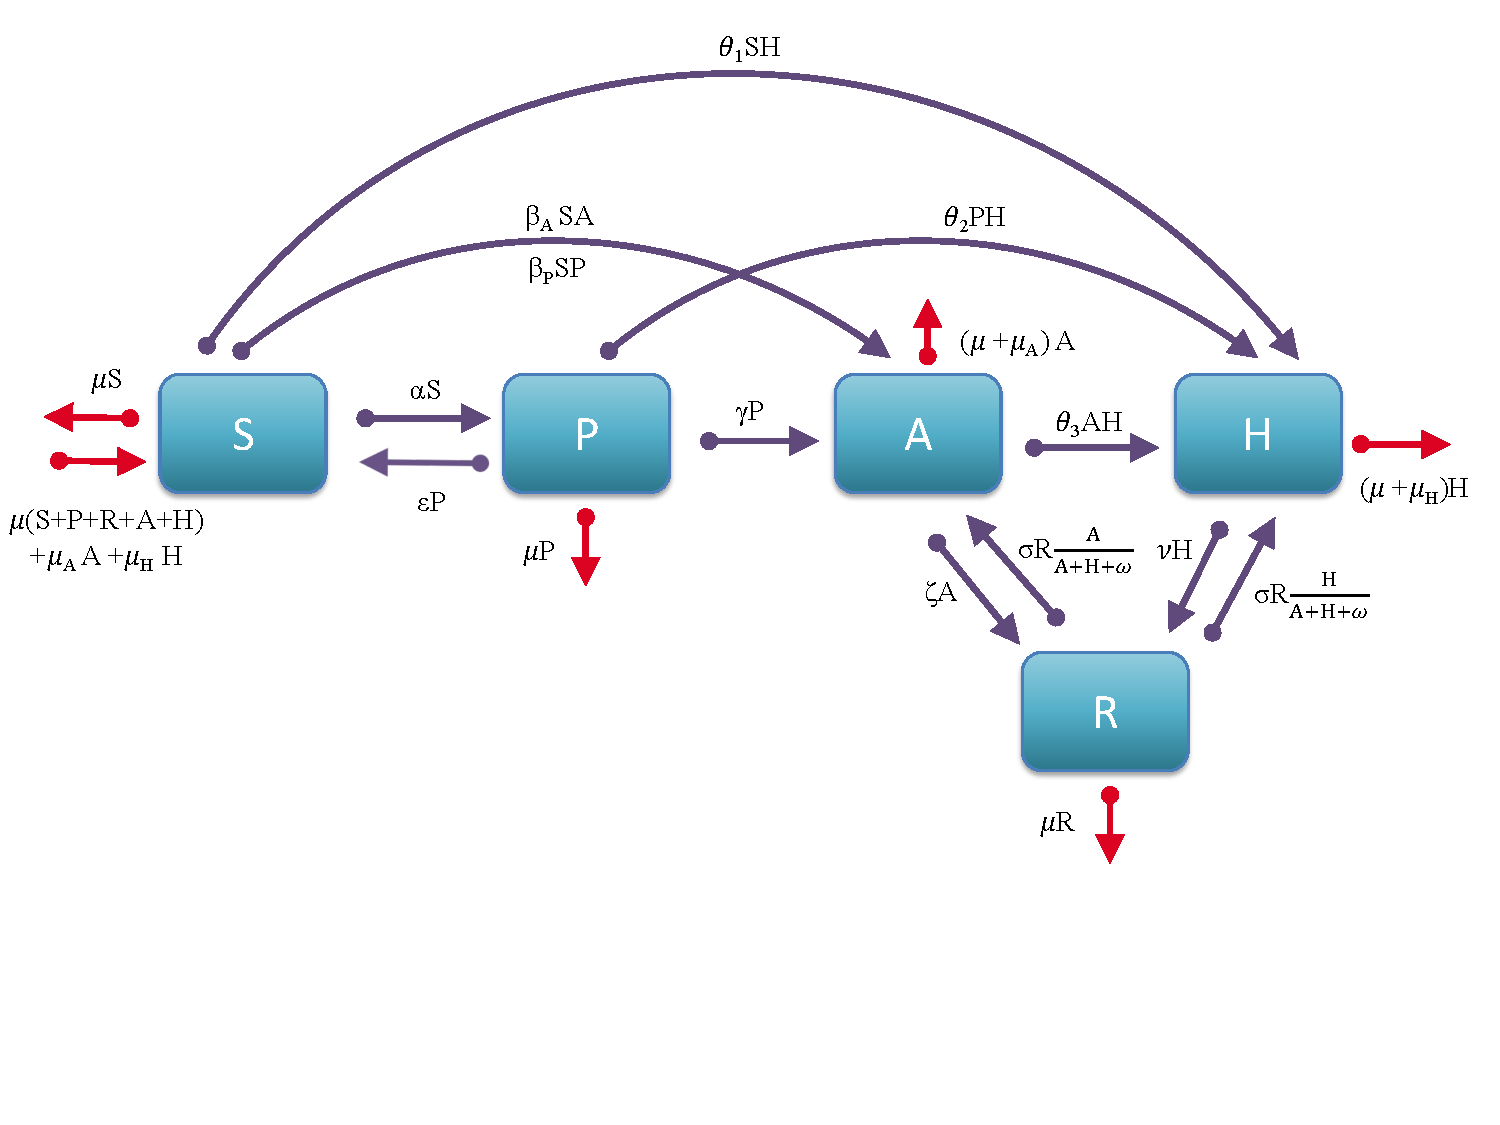
\includegraphics[scale=0.6]{heroin_schematic.pdf}
\vspace{-0.8cm}
\begin{center}
Figure 1: Schematic diagram for heroin model
\end{center}

%Christopher's words: (Regarding why we have so many assumptions). What can we say with a simple model? And from there, what can't we say? <-- This latter question gives us direction for how to improve the model and what we should do to build/extend the model further. 


\textbf{Analysis of the Model} \\ \\

 \textcolor{blue}{Addiction-Free Equilibrium} 

To find the addiction-free equilibrium, we set equations (1)-(5) equal to zero and require that $A=H=0$ since these two compartments consist of individuals who are addicted to opioids or heroin. We are left with the system: \\
\[0=-\alpha S^* -\beta_{P} S^* P^* + \epsilon P^* +\mu (P^* + R^*) \quad (7)\]
\[0=\alpha S^* - \epsilon P^* -\gamma P^* - \mu P^* \quad(8)\]
\[0=\gamma P^* + \beta_{P} S^* P^*.   \quad(9)\]
\[0=\mu R^* \quad(10)\]
\[1=S^*+P^*+A^*+H^*+R^* \quad(11)\]


Equation (10) forces either $\mu=0$ or $R^*=0$; however, $\mu > 0$ since this is the natural death rate, so we require $R^*=0$. If $P^* \neq 0, $ this forces $\gamma + \beta_{P} S^* =0$ from equation (9), and since all of our parameters and variables are non-negative, then it must be $\gamma=0$ and $\beta_{P}=0$. We note that $\gamma=0$ means that individuals who are prescribed opioids cannot become addicted to opioids, and $\beta_{P}=0$ means that only black market opioids are available for susceptibles to become addicted to opioids and there are no excess prescription drugs available. Under the assumption that $\gamma=0=\beta_{P}$ to ensure the existence of our addiction-free equilibrium, we calculate the addiction-free equilibrium to be: \\

\[S^*=\frac{\epsilon + \mu}{\alpha + \epsilon +\mu}\quad\]
\[P^*=\frac{\alpha}{\alpha + \epsilon +\mu}\quad\]
\[A^*=0\quad\]
\[H^*=0\quad\]
\[R^*=0\quad\] 

If $P^*=0$, then equation (8) forces either $S^*=0$ or $\alpha=0$.  If $S^*=0$, then the solution  $S^*=P^*=A^*=H^*=R^*=0$ contradicts equation (11). If $\alpha=0$, then we use equation (11) to solve for the addiction-free equilibrium of (1,0,0,0,0); this solution is included in the addiction-free equilibrium above when $\alpha=0$, as well. 

\textcolor{blue}{Basic Reproduction Number, \textbf{$\mathscr{R}_0$}}  
%Can numerically check R_0 (i.e. plug in specific values for F and V and make sure that matches my R_0). Make sure if R_0>1, goes away from my equilibrium and if R_0<1, goes toward my equilibrium. 

The basic reproduction number, denoted $\mathscr{R}_0$, is a term used in epidemiological models that gives the expected number of secondary disease cases that result from the introduction of a disease to a susceptible population. The value of $\mathscr{R}_0$ represents how successful the spread of the disease is expected to be; if $\mathscr{R}_0 < 1$, then the disease is expected to die out and the disease-free equilibrium will be locally stable; conversely, if $\mathscr{R}_0 >1$, then the disease is expected to spread and the disease-free equilibrium will be unstable \cite{Driessche}. \\ \\
 This idea may be applied to the context of our model since for the addiction-free equilibrium to occur, $\gamma$ and $\beta_{P}$ must both be equal to 0, which means individuals can become addicted only with interactions with opioid addicted individuals or heroin users so this takes the form of an infectious disease. Thus, in this case in which the prescription part is essentially taken out of the model so that it is a black-market-only driven model, $\mathscr{R}_0$ can be calculated. This value will be the ratio of the number of new addictions in the next year compared to the current year. At the addiction-free equilibrium, the population is completely susceptible, as needed for $\mathscr{R}_0$ to be an accurate measurement of addiction potential. 
We note that our goal in this section is to explore the structure of the model and not obtain a result for the full model. The disease compartments are those that contain infected individuals, or in our case, addicts \cite{Driessche}. Our model incorporates two addiction compartments, A and H, since these both consist of opioid or heroin/fentanyl addicted individuals. We will utilize the Next Generation Matrix Method in order to calculate $\mathscr{R}_0$.


For the purposes of calculating $\mathscr{R}_0$, we will assume $\gamma =0$ and $\beta_{P} =0$ in order to ensure the existence of the addiction-free equilibrium. This results in the following system:
\[\dv{S}{t} = -\alpha S - \beta_{A} SA  - \theta_{1} SH +\epsilon P +\mu (P+R) + (\mu+\mu_{A})A + (\mu+\mu_{H}) H \quad \] 
\[\dv{P}{t} = \alpha S - \epsilon P  - \theta_{2}PH- \mu P    \quad\]
\[\dv{A}{t} = \sigma R \frac{A}{A+H+\omega} +\beta_{A} SA  -\zeta A - \theta_{3}AH-(\mu + \mu_{A})A   \quad\]
\[\dv{H}{t} = \theta_{1}SH+\theta_{2}PH+\theta_{3}AH + \sigma R \frac{H}{A+H+\omega}-\nu H-(\mu+\mu_{H})H  \quad\]
\[\dv{R}{t} = \zeta A +\nu H -\sigma R \frac{A}{A+H+\omega}-\sigma R \frac{H}{A+H+\omega} -\mu R.\quad\]


In general, the differential equations of the $n$ disease compartments, $x_i'$, may be written as: 

\[{x_i'} = \mathscr{F}_{i} (x,y)-\mathscr{V}_i (x,y),\quad i=1,...,n\] 

where $x$ is a vector with the disease compartments as components, $y$ a vector with the non-disease compartments as components, $\mathscr{F}_{i}$ represents the rate that secondary infections contribute to disease compartment $i$ and $\mathscr{V}_{i}$ represents the rate of transitions, i.e. rate at which the disease compartment $i$ is decreased by means of death, recovery and progression of the disease for $i=1,2$ \cite{Driessche}. 

Thus, for our two addicted compartments, we may write: 

$$\dfrac{dA}{dt} = \mathscr{F}_{1} (x,y)-\mathscr{V}_{1}(x,y)$$
$$\dfrac{dH}{dt} = \mathscr{F}_{2} (x,y)-\mathscr{V}_{2}(x,y)$$

where $x= {[A\quad H]}^{T}$ and $y= {[S\quad P\quad R]}^{T}$.



Thus, under the assumption that A and H are the addicted compartments and abiding by the parameter restrictions stated above, the assumptions of the Next Generation Method are satisfied for matrices $\mathscr{F}$ and $\mathscr{V}$ formulated here:

\begin{center}
$\mathscr{F}=$
$ \begin{pmatrix}

\sigma R \frac{A}{A+H+\omega}+\beta_{A} SA \\
\theta_{1}SH+\theta_{2}PH+\sigma R \frac{H}{A+H+\omega} \\
\end{pmatrix}$



$\mathscr{V}=$
$ \begin{pmatrix}

\zeta A+\theta_{3} AH + (\mu +\mu_{A})A \\
-\theta_{3}AH+\nu H +(\mu +\mu_{H}) H \\
\end{pmatrix}$.
\end{center}

These assumptions include the following: 
\begin{itemize}
\item $\mathscr{F}_{i} (0,y)=0$ and $\mathscr{V}_{i}(0,y)=0$,  $\forall$$y \geq 0$, $i=1,2$, which ensures that new addictions arise only from interacting with those currently addicted, and there is no immigration into the addicted compartments; these guarantee that the population free of addiction remains that way. 
\item $\mathscr{F}_{i} (x,y) \geq 0$, $\forall$$x,y \geq 0$, $i=1,2$ since these represent new addictions. 
\item $\mathscr{V}_{i}(x,y) \leq 0$ whenever $x_i=0, i=1,2$ since there must be inflow only when the respective compartment is empty. 
\item $\sum_{i=1}^{2} \mathscr{V}_{i}(x,y) \geq 0$, $\forall x,y \geq 0$ since this represents the total outflow from all addicted compartments. 
\item The addiction-free system, $\dv{S}{t}\bigg|_{A,H=0}$, $\dv{P}{t}\bigg|_{A,H=0}$, and $\dv{R}{t}\bigg|_{A,H=0}$ has a unique equilibrium, ($\frac{\epsilon+\mu}{\alpha+\epsilon+\mu}$,$\frac{\alpha}{\alpha+\epsilon+\mu},0$) that is asymptotically stable. 
\end{itemize}

Taking $F=\frac{\partial \mathscr{F}_i}{\partial x_j} (0, y_0)$ and $V=\frac{\partial \mathscr{V}_i}{\partial x_j} (0, y_0)$, $i, j =1, 2$, where (0, $y_{0}$) $=(\frac{\epsilon + \mu}{\alpha + \epsilon +\mu},\frac{\alpha}{\alpha + \epsilon +\mu},0,0,0)$ is the addiction-free equilibrium, we calculated the following \cite{Driessche}: 



\begin{center}
$F=$
$ \begin{pmatrix}

\beta_{A} \frac{\epsilon+\mu}{\alpha+\epsilon+\mu} &  0  \\
0 & \theta_1 \frac{\epsilon+\mu}{\alpha+\epsilon+\mu}  +\theta_2 \frac{\alpha}{\alpha+\epsilon+\mu}  \\
\end{pmatrix}$



$V=$
$ \begin{pmatrix}

\zeta +\mu +\mu_A &  0  \\
0 &  \nu+\mu+\mu_H \\

\end{pmatrix}$.
\end{center}

The eigenvalues of $FV^{-1}$ are calculated to be: 
\begin{center}
$\sigma (FV^{-1}) = \{ \frac{\beta_A(\epsilon+\mu)}{(\alpha+\epsilon+\mu)(\zeta+\mu+\mu_A)}, \frac{\theta_1(\epsilon+\mu)+\theta_2 \alpha}{(\alpha+\epsilon+\mu)(\nu+\mu+\mu_H)} \}$
\end{center}

$\mathscr{R}_0$ may then be determined as the spectral radius of $FV^{-1}$, in which the $(i,j)$ entry is the expected number of secondary addictions in compartment $i$ produced by individuals initially in compartment $j$ :
\begin{center}
$\mathscr{R}_0=$ WHICHEVER IS LARGEST WHEN KNOW VALUES! 
\end{center}

\textcolor{blue}{Include proof of non-negative IC implies non-negative solutions?} \\ 
\textcolor{blue}{What other analysis should be done?} \\ \\

\textbf{Numerical Results} 
(literature information and parameter estimation) \\ \\
 
 \textcolor{green}{Data used within code} \\
 \textcolor{blue}{Applying model to Tennessee population} \\
 \textcolor{red}{This is where start to talk about Tennessee} \\
We apply our model to the Tennessee population specifically in order to analyze the opioid epidemic on a smaller scale than the national level. Although there is still heterogeneity across Tennessee, it is lower than the amount one would find on a national scale. Below we present a data table consisting of estimates of the number of individuals in Tennessee in various categories for the years 2013-2018 found either in literature or that we estimated; explanations of each of the categories follows. 

\textcolor{blue}{Leave data table/information here or put in appendix?}
\textcolor{red}{Put in information of US prescription rate per capita at it's peak was 81.3/100 people and how TN has been far above that every year.}
\captionof{table}{Number of individuals in each category, 2013-2018}
\begin{tabular}{|l|c|c|c|c|c|c|l}
\hline
 & \footnotesize{2013} & \footnotesize{2014} & \footnotesize{2015} & \footnotesize{2016} & \footnotesize{2017} & \footnotesize{2018}\\
\hline
\footnotesize
Total population & \footnotesize{6,490,795} & \footnotesize{6,540,007} & \footnotesize{6,590,726} & \footnotesize{6,649,404} & \footnotesize{6,715,984} & \footnotesize{6,770,010}\\
\footnotesize
Population 12 and older & \footnotesize{5,517,176} & \footnotesize{5,559,006} & \footnotesize{5,602,117} & \footnotesize{5,651,993} & \footnotesize{5,708,586} & -\\
\footnotesize
Prescription opioid users (includes those addicted) & \footnotesize{1,845,144} &\footnotesize{1,824,342} & \footnotesize{1,819,581} & \footnotesize{1,761,363} &  \footnotesize{1,636,374} &-\\
\footnotesize
Opioid addicts & \footnotesize{\textit{48,674}} & \footnotesize{\textit{48,163}} & \footnotesize{48,000
} & \footnotesize{42,000} & \footnotesize{\textit{39,020}} &-\\
\footnotesize
Non-addicted prescription opioid users   & \footnotesize{\textit{1,823,581}} &\footnotesize{\textit{1,803,006
}} & \footnotesize{1,798,317} & \footnotesize{1,642,757} &  \footnotesize{\textit{1,619,088
}} &-\\
\footnotesize
Heroin addicts & - &\footnotesize{14,000} & \footnotesize{14,000} & \footnotesize{19,000}  & - &-\\
\footnotesize
Prescription opioid overdose deaths & - & - & \footnotesize{679} & -  & - &-\\
\footnotesize
Heroin/fentanyl overdose deaths & - & - & \footnotesize{374} & -  & - &-\\
\footnotesize
Prescription opioid treatment admissions & \footnotesize{4,485} & \footnotesize{4,530} & \footnotesize{4,326} & -  & - &-\\
\footnotesize
Heroin treatment admissions & \footnotesize{555} & \footnotesize{743} & \footnotesize{1,083} & -  & - &-\\
\hline
\end{tabular} \\
\label{tab:template}


 \textcolor{blue}{Explanations of the estimates/where they come from in literature/assumptions made} \\ \\
 \textcolor{blue}{Some of these are data points that are used directly in parameter estimation code, but some are used for calculation of $\mu$, $\mu_A$, $\mu_H$, IC,...leave these explanations here or put them in the appendix?} \\
 First we note that the italicized values are numbers that we estimated, the rest are actual data. 
The first row provides the \textbf{total population estimates in Tennessee} each year \cite{USCensus}. However, since the remainder of the data we use is specific to individuals 12 and older, we estimate the number in this age group. 
There were an estimated 1,073,214 individuals in Tennessee in 2018 aged 12 and under. (Note: we could not find the estimate for this age group for the years 2013-2017, so this is the best estimate we have for this age group). To figure out those who are 12 years old, we take approximately 1/8th of the individuals that are in the age group 5-12, which is approximately 83,175 individuals \cite{DOHHS}. Thus, an estimated 990,039 individuals are \emph{under} the age of 12 in Tennessee. Given the total population estimate for 2018 being 6,770,010 from row 1, this means that approximately 15\% of the population is under the age of 12. Since we do not see a reason for this percentage to be significantly different from year to year, we assume that this percentage is constant throughout the time period we are looking at. Then, we are able to consider the \textbf{Tennessee population estimates for individuals 12 and older} in order to align with the rest of the data that is in this age range by taking off 15\% of the above total population estimates; this is shown in the second row.  \\

The \textbf{total number of individuals taking prescription opioids} for pain is given in the third row \cite{TNgov1}. Although this number does not explicitly state it is for individuals 12 and older, we assume it is since it comes from the Tennessee Department of Health; if it does include individuals under 12, we assume that number is negligible. \\

The 2015/2016 average number of individuals 12 and older with ``Pain Reliever Use Disorder" (\textbf{opioid addicts}) is 48,000 and the 2016/2017 average number was 42,000 \cite{NSDUH2, NSDUH3}. \textcolor{blue}{Right now, I'm using these estimates for the years 2015 and 2016...is that okay? I.e. for the ``average" data points, used the lowest of the two years} \textcolor{red}{May need to fill in more details about specific data such as collection process, self-reported probably equates to underreported, etc.}
We note that their definition of pain reliever use disorder includes those who meet the American Psychiatric Association criteria for dependence or abuse. Here, opioid dependence is classified as having "signs and symptoms that reflect compulsive, prolonged self-administration of opioid substances that are used for no legitimate medical purpose or...are used in doses that are greatly in excess of the amount needed for pain relief...regular patterns of compulsive drug use that daily activities are typically planned around obtaining and administering opioids." This definition falls under our definition of opioid addiction. Opioid abuse, on the other hand, they consider to be less severe than dependence, and would not lead to the development of withdrawal symptoms. This latter definition does not fall under our characterization of addiction, but we make a note of this to say that this estimate for those with a pain reliever use disorder may be overestimated for what we are concerned with, but is an acceptable approximation \cite{DSM}. In addition, we assume very few, if any, individuals are addicted to opioids outside of prescription opioids, but even if they are, we assume they are taking prescription opioids in some capacity, so we take pain reliever use disorder to include those with other non-prescription opioid addiction. We also remind the reader that these numbers include both individuals who are personally prescribed opioids or may obtain them illicitly.   \textcolor{red}{May find a better place for this later: Finally, we note that those who are addicted to opioids are strictly in the A class, as individuals in R are not considered addicted in our model.} 

From 2013 to 2017, the number of prescription opioid users was decreasing, probably due to more awareness of the problem as suggested in \cite{CDC7}, and thus, we expect the number of addicts to also be decreasing in that time period, especially due to the movement of individuals to heroin use. For 2015, we see there were 48,000 opioid addicts compared to 1,819,581 prescription opioid users, which is an approximate ratio of 1:37.9; thus, we use this exact ratio of addicts to prescription opioids users for 2013 and 2014, as well, to estimate the number of opioid addicts (these values are in italics in Table 1). Although the numbers are most likely higher than this, this is an estimate. We apply a similar idea for the year 2017, utilizing data from 2016 that there are 42,000 opioid addicts out of 1,761,363 prescription users, which is an approximate ratio of 1:41.9. 
%Calculations: 
%For 2015: 1819581/48000=37.9079375 so for 
%2013: 1845144/37.9079375=48674
%2014: 1824342/37.9079375=48163
%For 2016: 1761363/42000=41.93721429 so for
%2017: 1636374/41.93721429=39020 

The total number of prescription users each year, however, includes individuals addicted to their prescriptions. In a 2015 study done among adults with prescription opioid use disorder, 44.3\% of them had obtained prescription opioids for their most recent episode of misuse from 1 or more physicians \cite{Han}. Therefore, we assume that 44.3 out of 100 addicts are personally prescribed opioids and subtract 44.3\% of the number of addicts in each year from the prescription opioid class in the corresponding year to obtain the number of non-addicted prescription opioid users for 2013-2017. We assume here that individuals who use heroin are not using \textit{prescribed} opioids, since they are more expensive and provide less of a high, and therefore, heroin addicts do not need to be factored out of these total numbers. \\
%Calculations:
%In 2013, 48674*0.443=21563 so 1845144-21563=1823581
%In 2014: 48163*0.443=21336 so 1824342-21336=1803006
%In 2015: 48000*0.443=21264 so 1819581-21264=1798317
%In 2016: 42000*0.443=18606 so 1761363-18606=1642757
%In 2017: 39020*0.443=17286 so 1636374-17286=1619088
The 2014/2015 average number of individuals 12 and older with ``Past Year Heroin Use" (\textbf{heroin/fentanyl addicts}) was 14,000, the 2015/2016 average number was 14,000, and the 2016/2017 average number was 19,000 \cite{NSDUH0, NSDUH2, NSDUH3}. \textcolor{blue}{Right now, I'm using these estimates for the years 2015 and 2016...is that okay?}  Although this number includes those who may have used heroin once or twice in the past year, we are under the assumption that the majority of these individuals are addicts and that very few, if any, individuals use heroin recreationally. In addition, the number of heroin users does not include fentanyl users explicitly, but we are under the assumption that those who take fentanyl are a subset of those who use heroin, and therefore, would mostly be included in these numbers. We admit the values may be slightly too low, for the cases of individuals who do fentanyl and not heroin, but data has not been found for fentanyl addicts only. Therefore, we are working under the assumption that it would be a negligible population that takes fentanyl without heroin. Overall, these two assumptions may work to balance one another out. \\

We use data on the number of prescription opioid overdose deaths which include natural, semi-synthetic, and synthetic opioids; however, we subtract out the number of fentanyl overdoses (fentanyl is classified as a synthetic prescription opioid), since those overdoses are counted for in their own category, listed below. This results in (848-169=) 679 as the \textbf{total number of prescription opioid overdose deaths} for 2015. \cite{PDO}. Although this number does not explicitly state it is for individuals 12 and older, we assume it is since it comes from the Tennessee Department of Health; if it does include individuals under 12, we assume that number is negligible. \\

We add together the heroin and fentanyl overdoses for the state of Tennessee to obtain the \textbf{total number of heroin and fentanyl overdoses} in 2015 to be (205+169=) 374 \cite{PDO}. Although this number does not explicitly state it is for individuals 12 and older, we assume it is since it comes from the Tennessee Department of Health; if it does include individuals under 12, we assume that number is negligible. \\

For Tennessee individuals 12 and older, \textbf{the number of treatment admissions for non-heroin opiates/synthetics} as the primary substance of abuse to facilities that receive state/public funding (generally referring to funding by the state substance abuse agency) is found in row eight of Table 1 \cite{TEDS2015_SAMSHA_admissions}. Here, we take non-heroin opiates/synthetics to mean prescription opioids. We are under the assumption that if one were addicted to heroin in addition to prescription opioids, their heroin problem would be the primary reason for going to treatment and would be included in the following numbers. Finally, row nine of Table 1 gives the \textbf{number of treatment admissions} for heroin as the primary substance of abuse to facilities that receive state/public funding (generally referring to funding by the state substance abuse agency) for Tennessee individuals 12 and older \cite{TEDS2015_SAMSHA_admissions}. Again, these numbers do not include fentanyl users explicitly, but we are under the assumption that those who take fentanyl are a subset of those who use heroin, and therefore, would mostly be included in these numbers. We admit the values may be slightly too low, for the cases of individuals who do go to treatment with the primary substance of abuse being fentanyl, but there is not data available for those numbers currently. 


Calculations of parameters and estimates of initial conditions from this data is found in Appendix A. \\



\textcolor{blue}{Parameter estimation process} \\
The age-adjusted death rate ($\mu$) and overdose death rates ($\mu_{A}$ and $\mu_{H}$) are calculated and assumptions on $\theta_2$, $\theta_3$, $\beta_A$, and $\beta_P$ are stated in Appendix A. In addition, although we have an estimate for the total number of prescription opioid users and opioid addicts in 2013, we do not know these numbers at the start of 2013; similarly for the other states. Thus, we approximate the initial conditions of our states for 2013 in Appendix A using information from Table 1. 

\begin{center}

\begin{tabular}{|c | c | c|}

 \hline

{Parameter} & {Value Assumed} & {Units} \\ [0.5ex]

 \hline\hline

$\beta_A$ &  &  \\

\hline

$\beta_P$&  &  \\

\hline

$\theta_2$ &  &  \\

\hline

$\theta_3$ &  &  \\

\hline


$P_0$ &  &  \\

\hline

$A_0$ &  &  \\

\hline

$H_0$ &  &  \\

\hline

$R_0$ &  &  \\

\hline
\end{tabular}

\end{center}
 


In order to estimate the remaining parameters for our model, we utilized the ordinary least squares method and formulated an objective function to minimize, which consists of the squared differences between data and model simulations. We have data on the total number of non-addicted prescription users, opioid addicts, and heroin/fentanyl addicts each year, and therefore on their corresponding proportions out of the entire population in a given year. We have data on the proportion of individuals in P at some point during each of the years 2013-2017, the proportion of individuals in A at some point during each of the years 2014-2015, and the proportion of individuals in H at some point during each of the years 2014-2016, resulting in a total of 10 data points. \\

\textcolor{blue}{Include these next couple of descriptions in paper or only in dissertation?} \\
We simulate the proportions in each of these classes throughout the year in the following way. 
In order to count the proportion of individuals in P, A, or H at some point throughout a certain year, 
 we need to count those who are in each of the classes AT ALL during the year, even if they leave or come back at some point. We note that we neglect higher order terms, i.e. people who go into the P class multiple times, since we can't keep track of individuals in model; the data we use is about total proportion of people who are in the class at some point throughout the year but they are kept track of and only counted once. \\
  
To get the output from the model of the proportion of non-addicted prescription opioid users in each year, we take the proportion of non-addicted prescription opioid users at the beginning of each of the years and add on the proportion of individuals that enter the P class at any point during the year. This latter part comes from integrating over those who enter the P class: $\int_0^t X'(t)dt=\int_0^t \alpha S(t)dt$ which is equal to $X(t)-X(0)$; here, we take $X(0)=0.$ For every year except 2013, a subtraction must be done since integrating gives the proportion from time $0$ to time $t$, but we only want the proportion from time $t-1$ to time $t$ (i.e. the new cases in a given year). Thus, the calculation is as follows for each year, with the last equation in each line what was calculated in the code: \\
2013: $P_0 + \int_0^1 \alpha S = y(1,2)+y(2,6)-y(1,6)$ \\
2014: $y(2,2)+\int_1^2 \alpha S$=$y(2,2)+\int_0^2 \alpha S$- $\int_0^1 \alpha S=y(2,2)+y(3,6)-y(2,6)$ \\
2015: $y(3,2)+\int_2^3 \alpha S$=$y(3,2)+\int_0^3 \alpha S$- $\int_0^2 \alpha S=y(3,2)+y(4,6)-y(3,6)$ \\
2016: $y(4,2)+\int_3^4 \alpha S$=$y(4,2)+\int_0^4 \alpha S$- $\int_0^3 \alpha S=y(4,2)+y(5,6)-y(4,6)$ \\
2017: $y(5,2)+\int_4^5 \alpha S$=$y(5,2)+\int_0^5\alpha S$- $\int_0^4 \alpha S=y(5,2)+y(6,6)-y(5,6)$ \\


 To get the output from the model of the proportion of opioid addicts in 2014 and 2015, we take the initial proportion of opioid addicts in each of these years and add the proportion of individuals that enter the A class at any point during the year 2014 or 2015. This latter part comes from integrating over those who enter the A class: $\int_0^t L'(t)dt=\int_0^t (\gamma P + \sigma R\frac{A}{A+H+\omega}+\beta_A SA+\beta_P SP) dt$ which is equal to $L(t)-L(0)$; here, we take $L(0)=0.$ Similar to above with the subtraction of integrals to calculate for a specific year, we have: \\
 2014: $y(2,3)+\int_1^2 (\gamma P + \sigma R\frac{A}{A+H+\omega}+\beta_A SA+\beta_P SP) dt= y(2,3)+y(3,7)-y(2,7)$ \\
 2015: $y(3,3)+\int_2^3 (\gamma P + \sigma R\frac{A}{A+H+\omega}+\beta_A SA+\beta_P SP) dt= y(3,3)+y(4,7)-y(3,7)$ \\


Finally, to obtain the output from the model of the proportion of heroin/fentanyl addicts for each year 2014-2016, we take the initial proportion of heroin/fentanyl addicts in each of these years and add the proportion of individuals that enter the H class at any point during the year. This latter part comes from integrating over those who enter the H class: $\int_0^t M'(t)dt=\int_0^t (\theta_1 SH+\theta_2 PH+\theta_3 AH +\sigma R \frac{H}{A+H+\omega})dt$ which is equal to $M(t)-M(0)$; here, we take $M(0)=0.$ Similar to above with the subtraction of integrals to calculate for a specific year, we have: \\
 2014: $y(2,4)+\int_1^2  (\theta_1 SH+\theta_2 PH+\theta_3 AH +\sigma R \frac{H}{A+H+\omega}) dt= y(2,4)+y(3,8)-y(2,8)$ \\
 2015: $y(3,4)+\int_2^3  (\theta_1 SH+\theta_2 PH+\theta_3 AH +\sigma R \frac{H}{A+H+\omega}) dt= y(3,4)+y(4,8)-y(3,8)$ \\
 2016: $y(4,4)+\int_3^4  (\theta_1 SH+\theta_2 PH+\theta_3 AH +\sigma R \frac{H}{A+H+\omega}) dt= y(4,4)+y(5,8)-y(4,8)$ \\


We use the Global Optimization Toolbox in MATLAB, specifically utilizing the MultiStart algorithm and fmincon local solver. Since we wish to know the global minimum, we use \textcolor{red}{fill in number} starting points as this is a local solver. We give lower bounds of 0.00001 for all of the parameters and an upper bound of 2 for all of the parameters except $\epsilon$ with an upper bound of 4 since this parameter can easily be greater than 1 (i.e. in a given year, a prescription user may end prescription use more than once). We run our model from 2013-2018, keeping a short time frame so that dynamics are relatively the same in the time period with the time step in years. 

\textcolor{blue}{How many details to give for paper? Put in anything needed for paper from MatLab\_descriptions.pdf if applicable.}


%I tried to choose realistic lower and upper bounds for the parameters in the following way: $\alpha$ guess from opioid paper since higher in TN; $\beta_A $ guess from opioid paper; 
 %$\beta_P$ guess from opioid paper; $\theta_1$ complete guess, assume smaller than $\beta_A$, $\beta_P$; 
% epsilon 0.8-8 from opioid paper; gamma guess from opioid paper; $\theta_2$
% guess twice as large as $\theta_1$; $\sigma$ guess small because
% ``successful recovereds"; $\zeta$ will be smaller than opioid paper because fewer people will ``relapse" since more ``stable recovered" but still
% put opioid largest value in; $\theta_3$ guess four times as large as
% $\theta_1$; $\nu$ guess same as $\zeta$; $P_0$
% guess; $A_0$ guess; $H_0$ guess; $R_0$ guess} \\ \\


The following table displays the 7 parameters that were estimated with this process, along with their resulting estimated values: 



\begin{center}

\begin{tabular}{|c | c | c|}

 \hline

{Parameter} & {Estimated Value} & {Units} \\ [0.5ex]

 \hline\hline

$\alpha$ &  &  \\

\hline

$\theta_1$&  &  \\

\hline

$\epsilon$ &  &  \\

\hline

$\gamma$ &  &  \\

\hline


$\sigma$ &  &  \\

\hline

$\zeta$ &  &  \\


\hline

$\nu$ &  &  \\

 \hline

\end{tabular}

\end{center}
 






 
\textbf{Conclusions} \\ \\
 \textcolor{red}{What did we show that we didn't know before?} \\
 \textcolor{red}{Think of questions that we can confront the model with regarding heroin and fentanyl deaths and connect to data on deaths; give results that give the reader an answer to these questions; think about analysis can do on model.} \\
 
 \textcolor{blue}{Extensions}\\
 \textcolor{red}{Need to edit} \\
In our model we assume homogeneous mixing of the individuals in each of the compartments and therefore, each individual has the same probability of transitioning from one stage to another, interacting with individuals from other stages, or leaving the system via death. Although done for the purpose of simplification, this is not an accurate representation of reality since there are factors that affect these probabilities, such as race, gender, geographical location and age. For example, there has been a shift in heroin use from urban areas to some suburban and rural areas and there is an increasing number of individuals ages 18-25 using the drug \cite{NIDA2}. West Virginia, New Hampshire and Ohio had the highest rates of opioid-related overdose deaths per 100,000 people in 2016 and Tennessee and Arkansas were among the states with the highest prescription rates per 100 people the same year \cite{NIH3}. Men have a higher likelihood of overdosing on prescription pain relievers compared to women, but since 1999, there has been a steeper increase in the number of women overdoses than men. In addition, women may form a quicker dependence on opioids compared to men, and have a higher probability of being prescribed higher doses and for longer periods of time \cite{CDC5}. Specific to heroin, using data from the 2008-2010 NSDUH studies, past year heroin use was twice as likely for men compared to women, and highest in the 18-25 year old age group \cite{Jones}. Incorporating these ideas into the model and parameter information would be possible future extensions. Although there is data on the misuse of opioids, we decided to focus specifically on addiction rather than misuse, due to the harmful consequences this behavior can have for an individual. However, the behavior and actions of individuals are not always very clearly defined, and there may be a benefit to expanding the spectrum of classes that individuals can fall into. 


\textbf{Appendix A} \\ \\
\textcolor{blue}{Calculations of parameters from literature} \\
%Could be helpful if need for individuals under 12: https://factfinder.census.gov/faces/tableservices/jsf/pages/productview.xhtml?src=CF 
The \textbf{age-adjusted death rate} for Tennessee in 2016 was calculated to be 886.3 out of 100,000 individuals, or approximately 50,094 people out of a total population 12 and older of 5,651,993 \cite{Kaiser}. Subtracting off the number of people who died from a prescription opioid or heroin/fentanyl overdose in 2016 results in 48,825 people who died that year. This implies that (5,651,993-48,825)/5,651,993 $\approx$ 0.991 is the proportion of the population that remains by the beginning of 2017. If we consider $T_0$ to be the total population in 2016, we can find the continuous-time rate at which individuals die naturally from the equation 0.991$T_0$=$T_0e^{-\mu t}$, which results in the natural death rate $\mu \approx 0.00868$.



%SEE WORK on 11/19/18 meeting notes for mu_A, mu_H, mu
We may calculate the overdose death rate in the year 2015, since we know the number of addicted individuals in that year. To find the continuous-time rate at which individuals are dying from the addicted class, we consider the equation $k A_{0}=A_{0}e^{-\mu_{A}t}$, where $A_0$ is the number of individuals addicted to opioids in 2015 and $k$ is the proportion of these individuals in the addicted class at the start of 2016 (when $t=1$). In 2015, there were 679 individuals out of the entire Tennessee population 12 and older that overdosed on prescription opioids \cite{PDO}. However, it is estimated that only 54.6\% of these individuals were actually at an increased risk for an opioid-related overdose death; we assume that if an individual met the criteria for at least one high-risk factor, that they were considered addicted to opioids \cite{Gwira}. Therefore, we assume 54.6\% of the 679 individuals that overdosed were addicted. With a total of 48,000 opioid addicts in 2015, this means that (48,000-0.546$\cdot$679)/48,000 $\approx$ 0.992 is the proportion of addicted individuals that remain by the beginning of the next year. This implies 0.992$A_0=A_0 e^{-\mu_{A}(1)}$, and solving results in \boldmath{$\mu_{A} \approx 0.00775.$}\unboldmath
%have to do this calculation because mu_A is IN the A class and not just anyone who overdoses 

Similarly, we may calculate $\mu_{H}$. There were 14,000 heroin/fentanyl addicts in 2015 and 374 heroin-related overdoses. We make the assumption that if an individual died of a heroin overdose they were addicted in line with our previous assumptions that if one is using heroin, they are considered addicted due to the nature of the drug. This means that (14,000-374)/14,000 $\approx$ 0.973 is the proportion of heroin users that remain at $t=1$, which implies 0.973$H_0=H_0 e^{-\mu_{H}(1)}$, which results in \boldmath{$\mu_{H}$ $\approx 0.0271$} \unboldmath, the continuous-time rate at which individuals are dying from the heroin class.

%we view it as a good thing that methadone was pulled out separately from this data for overdoses, because it's used in treatment in order to reduce cravings and not necessarily supply the high 

We make a note that individuals that do not have an opioid use disorder and die because of an opioid overdose are counted in the ``natural mortality rate." 

\textcolor{blue}{Estimates of parameters from literature} \\
Since there is no information for values of $\theta_1$, $\theta_2$, or $\theta_3$ for Tennessee in the literature, we consider a national study of individuals 12 and older to establish a relationship among these three rates. For a national study consisting of 609,000 participants, ``the recent heroin incidence rate was 19 times higher among those who reported prior non-medical pain reliever (NMPR) use (0.39\%) than among those who did not report NMPR use (0.02\%) \cite{Muhuri}.
NMPR use can occur within the prescription class (i.e. from misuse that's not considered addiction), or in the addiction class. Thus, we will extrapolate this information to say that the rate that prescription opioid users and opioid addicts move to heroin use is 19 times greater than the rate at which susceptibles move to heroin use (i.e. $\theta_2 + \theta_3$ $>$ 19$\theta_1$), where both $\theta_2$ and $\theta_3$ are greater than $\theta_1.$ We will make an assumption here that $\theta_2 + \theta_3$ is exactly 19$\theta_1$, and that there is somewhat of an elevated risk of moving to heroin use from the prescription class versus the susceptible class, taking $\theta_2 =3 \theta_1$. This leaves $\theta_3=16\theta_1.$ \\

\textcolor{blue}{Okay to use even though opioid model is not a sub-model anymore (since we've changed the recovery class and terms?} We argue that $\beta_A$ is a reasonable parameter to estimate because the opioid-only model was insensitive to this parameter and although less so, $\beta_P$ was relatively insignificant compared to other parameters explored \cite{Battista}. We were not able to find values in the literature specific to Tennessee regarding an illicit-induced addiction rate; however, we use information from the national level, as we do not have any evidence that this national average rate would be significantly different in Tennessee. \textcolor{blue}{Have this work checked/all units okay?} In 2015, there were an estimated 2.1 million individuals 12 and older that initiated pain reliever misuse recently. Using this source, we take pain relievers to be equivalent to prescription opioids \cite{SAMSHA5}. To calculate approximately how many of these would end up having a use disorder in 2015, this same study states that 12.5 million people misused prescription opioids in the past year total, and that there were 2.0 million with a prescription opioid disorder; using these number, we make an estimate that \\
$$\frac{2 \text{ million people with pain reliever use disorder in 2015}}{12.5 \text{ million people who misused pain relievers in 2015}}=0.16.$$
We extrapolate this to estimate that 16\% of the 2.1 million recent initiates are those who should be counted in the use disorder category (although we do not know the timeline of developing the use disorder and it may not happen within the year, it gives a rough idea). This results in an estimate of 336,000 individuals that were recent initiates of pain reliever misuse that we will consider having a use disorder within the year 2015. In the same year, a study was done regarding the source of the most recent episode of misuse of prescription opioids among adults reporting an prescription opioid use disorder in the past year \cite{Han}. (Note: this study was for individuals age 18 and older whereas the study done in \cite{SAMSHA5} was for those 12 and older; we will assume for simplicity that the information for those 18 and older will be similar to those between 12 and 18, as well.) Here, 52.8\% of the prescription opioids were from a non-physician source, which included being given to/bought from a friend/relative, or bought from a drug dealer/stranger. For simplicity, let IPUD indicate individuals with a prescription use disorder. 
Thus, \\
$$\frac{336,000\text { IPUD}}{320 \text{ million people}}\cdot \frac{0.528 \text{ source of opioids for IPUD is illicit}}{\text{all sources of opioids}}=$$
$$0.00105 \frac{ \text { IPUD obtain opioids illicitly}}{{\text{all opioid sources for entire population}}}.$$

In our model, we consider two cases in which individuals become addicted. From \cite{Han}, we see that \\
$$\frac{.138 \text{ opioids obtained from drug dealers/strangers by IPUD}}{.528 \text{ opioids obtained illicitly by IPUD}}=.26$$ 
relates to individuals obtaining opioids by the black market or interaction with other addicts and
$$\frac{.218+.141+.031 \text{ opioids given/bought from a friend/relative or other for IPUD}}{.528 \text{ opioids obtained illicitly by IPUD}}=.74$$ 
relates to individuals obtaining opioids from extra prescriptions that are available. 

Thus, 
$$\frac{0.26 \text{ opioids from drug dealers/strangers for IPUD}}{\text{ opioids obtained illicitly by IPUD}}\cdot \frac{0.00105 \text{ opioids obtained illicitly by IPUD}}{\text{all opioid sources for entire population}}$$
$$ =\frac{0.000273 \text{ opioids from drug dealers/strangers for IPUD}}{\text{all opioid sources for entire population}}$$
is the rate that individuals illicitly obtain their prescription opioids from the black market/other addict interaction and become addicted, $\beta_A$ and 
$$\frac{0.74 \text{ opioids from friend/relative or other by IPUD}}{\text{ opioids obtained illicitly by IPUD}}\cdot \frac{0.00105 \text{ opioids obtained illicitly by IPUD}}{\text{all opioid sources for entire population}}$$
$$ =\frac{0.000777 \text{ opioids from friend/relative or other for IPUD}}{\text{all opioid sources for entire population}}$$
is the rate that individuals illicitly obtain their prescription opioids from extra pills that are available and become addicted, $\beta_P.$ 



%Note, the numbers that are not cited have come from Table 1 and cited before. 
\textcolor{blue}{Estimates of initial conditions from literature} \\
There were 1,845,144 total individuals 12 and older who were prescribed opioids (which includes those addicted) at some point during 2013 
and there was an average of 1.271 prescriptions per person, although we will assume this number holds when only considering the age group 12 and older \cite{CDC6}. 
Thus, we calculate 
$$\frac{1.271 \text{ prescriptions}}{\text{person$\cdot$ year}}\cdot \frac{5,517,176 \text{ people}}{1,845,144 \text{ prescription users}} \approx \frac{ 3.80 \text{ prescriptions}}{\text{prescription user $\cdot$ year }}.$$  
In 2013, the average number of days of supply per prescription at the national level was approximately 16.5 days \cite{CDC7}.
Thus, this means there are 
$$\frac{3.80 \text{ prescriptions}}{\text{prescription user $\cdot$ year}} \cdot \frac{{16.5 \text{ prescription days}}}{\text{prescription}} \approx \frac{62.71 \text{ prescription days}}{\text{prescription user $\cdot$ year}} $$
which is approximately one sixth of the year. Therefore, we make a rough estimate that one sixth of the total number of prescription users throughout 2013 were using prescription opioids at the beginning of the year. %i.e. group these individuals into "6 groups" of 65 days each (although it doesn't work like that, but pretend 1/6th of the group has their 65 days starting from the beginning of the year, next 1/6th group for the next 65 days, and so on. 
 This gives our estimate of 
$$\frac{1,845,144 \text{ prescription users}}{\text{year}} \cdot \frac{1}{6} \text{ year} \approx 307,524 \text{ prescription users}$$
at the beginning of the year. Thus, 
$$\frac{307,524 \text{ prescription users}}{5,517,176 \text{ people}} \approx 0.056 $$
of the population was using opioid prescriptions at the beginning of 2013. 
Assuming, as before, a ratio of prescription users to opioid addicts in 2013 being approximately 1:37.9, we assume this is the ratio at the beginning of the year, as well, and so we have that $A_0=0.00148.$ As before, only 44.3\% of addicts are prescription users, so we take .443(.00148)$=$0.00065 and subtract this from the initial condition of P so that it correctly counts only non-addicted prescription opioids users: $P_0=0.056-0.00065=0.0553$ \cite{Han}. %explanation below data table above 
\\ \\

We do not have information on the number of heroin users in 2013, so we extrapolate from information in 2015. We note first that although opioid overdose deaths increase from 2013 to 2015, that does not necessarily equate to more heroin users in 2015, due to the rise in fentanyl contamination during this time period \cite{CDC4}. In order to keep a proportion approximately equivalent to the number of opioid addicts to heroin users in 2015, we assume the same ratio of approximately 1:3.43 heroin users to opioid addicts in 2013, as well. In 2013, addicts make up 0.00148 of the population at the start of 2013, so we assume $H_0 \approx 0.000431.$ (Note: the proportion of prescription opioid users to heroin users is also similar, particularly regarding the order of magnitude expected.) 
%This proportion seems plausible because we assume that a majority of individuals using heroin in 2015 are using the drug at the beginning of the year, since heroin is such an addictive substance and the only ways to leave the compartment are through dying or becoming stably recovered. If we take 75\% to mean the majority, we also arrive at $$\frac{0.75 \cdot 14,000 \text{ heroin users}}{5,602,117 \text{ individuals in population}} \approx 0.0019$$ as the proportion of heroin users at the beginning of 2013. 

Before, we estimated 48,674 opioid addicts in 2013; this higher number is supported by an overall higher prescribing rate in 2013 compared to the next few years \cite{CDC7}.
We will assume the number of heroin users is the same in 2013 as in 2014 and 2015. There were 4,485 prescription opioid treatment admissions and 555 heroin treatment admissions in 2013, which is 0.057 of the opioid addict and heroin user population combined that are in recovery. Only 35\% of those in treatment do not relapse within 4 weeks after treatment, and thus have the ability to be in R, which is approximately .0804 of the entire A+H class \cite{Bailey}.
Since 90\% of individuals relapse within one year post-treatment, that means that an additional 55\% relapse after the 4 week mark and move out of R; therefore, we make a simplifying assumption that 10\% of those that can be in R actually are at a specific point in time, resulting in a proportion of .00804 of addicted and heroin users total \cite{Bailey}. This equates to approximately 504 individuals, which out of a total population 12 years and older in 2013 of 5,517,716, we conclude $R_0=0.000091.$ \\


\pagebreak
\textcolor{blue}{Table of parameter values and units of parameters/unit conversions from data to parameters in parameter estimation} \\
\textcolor{red}{Fill in}


\begin{center}

\begin{tabular}{|c | c | c|}

 \hline

{Parameter} & {Unit Conversions} & {Units} \\ [0.5ex]

 \hline\hline
 
 $\mu$ &  &  \\

 \hline
 
 $\mu_A$ &  &  \\

 \hline
 
 $\mu_H$ &  &  \\

 \hline

$\alpha$ &  &  \\

 \hline

$\beta_A$ &  &  \\

\hline

$\beta_P$ &  &  \\

\hline

$\theta_1$&  &  \\

\hline

$\epsilon$ &  &  \\

\hline

$\gamma$ &  &  \\

\hline

$\theta_2$ &  &  \\

\hline

$\sigma$ &  &  \\

\hline

$\zeta$ &  &  \\

\hline

$\theta_3$ &  &  \\

\hline

$\nu$ &  &  \\

\hline

$P_0$ &  &  \\

\hline

$A_0$ &  &  \\

\hline

$H_0$ &  &  \\

\hline

$R_0$ &  &  \\

%\\ [1ex]

 \hline

\end{tabular}

\end{center}
 






\pagebreak

\bibliography{HeroinModel}

 \end{document}

